\section{Design of \sys}
\label{s:impl}

\sys is a coverage-directed concurrency fuzzer to effectively discover
concurrency bugs.
%
The key improvement of \sys lies in adopting interleaving segment
coverage and the coverage-directed interleaving search strategy
described in \autoref{s:design}.
%

In particular, \sys consists of two stages of fuzzing similar with
recent concurrency fuzzers, Razzer~\cite{razzer} and
Snowboard~\cite{snowboard}.
%
The first stage is a single-thread fuzzing, which focuses on
identifying two system calls that may expose new interleaving
segments.
%
The second stage is a multi-thread fuzzing to explore thread
interleavings and discover concurrency bugs.
%
In both stage, \sys traces memory accesses executed by each system
call to track\dr{} interleaving segments.
%
And in the the second stage, \sys adopts a mechanism to control thread
scheduling as desired.



In the following of subsections, we provide the overall design of
\sys~(\autoref{ss:fuzzer}).
%
Then, we describe the target kernel
instrumentation~(\autoref{ss:instrumentation}) to trace memory
accesses and the execution engine~(\autoref{ss:engine}) to control
thread schedulings, followed by the implementation detail of
\sys~(\autoref{ss:impl}).




\subsection{Userspace Fuzzer}
\label{ss:fuzzer}



\begin{figure}
  \centering
  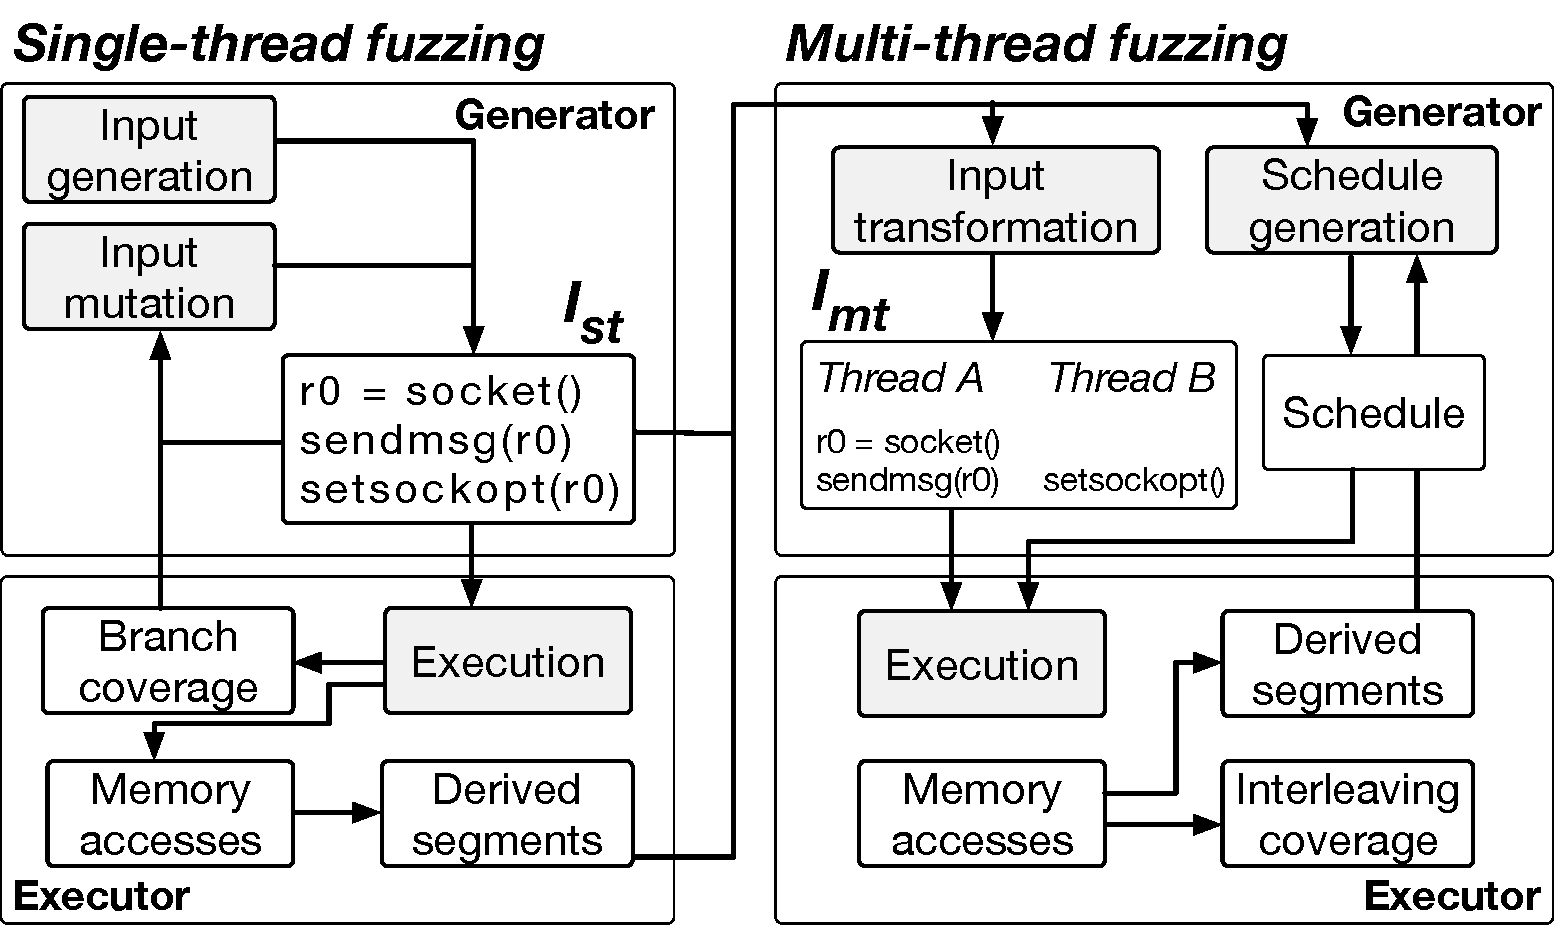
\includegraphics[width=0.9\linewidth]{fig/architecture.pdf}
  \caption{An overview of \sys.}
  \label{fig:workflow}
\end{figure}


In \sys, both single-thread fuzzing multi-thread fuzzing consist of
two components, an input generator and an input executor. We explain
details of each component in the following.


\subsubsection{Single-thread fuzzing}
\label{ss:singlethreadfuzzing}
%
In a single-thread fuzzing stage, the single-thread generator
generates a single-thread input (refered as $I_{ST}$) in the form of a
sequence of random system calls.
%
And then, the single-thread executor executes $I_{ST}$ to perform two
things.
%
First, it tracks code coverage of $I_{ST}$ as conventional fuzzing
does.
%
Second, it identifies two system calls in $I_{ST}$ that potentially
exhibit new interleaving segment coverage.  If identified, $I_{ST}$
will be passed to the next stage, the multi-thread fuzzing.


\PP{Single-Thread Generator}
%
The single-thread generator is similar with conventional
fuzzing~\cite{syzkaller}.
%
It constructs a single-threaded system call sequence $I_{ST}$ with two
strategies: generation and mutation.
%
When using the generation strategy, \sys randomly generates a system
call sequence based on well-formed system call description grammar
\texttt{Syzlang}~\cite{syzlang}.
%
\texttt{Syzlang} describes templates of available system calls
including types of arguments and the type of a return value, as well
as a range of feasible values of each arguments.
%
According to \texttt{Syzlang}, \sys produces a single-thread system
call sequence by repeatedly selecting a random system call and
providing reasonable arguments of the system call.

The mutation strategy is an alternative of the generation strategy.
When using a mutation strategy, \sys picks up a already-generated
single-thread input, and modifies the single-thread input by appending
additional system calls, removing existing system calls, or changing
values of arguments of existing system calls.


\PP{Single-Thread Executor}
%
Given $I_{ST}$ from the single-thread generator, the single-thread
executor runs $I_{ST}$, and traces basic blocks and memory accesses
executed by each system call with a support from instrumentation
detailed in \autoref{ss:instrumentation}.

With traced basic blocks and memory accesses, the single-thread
executor conducts two tasks.
%
The first task is similar with what conventional kernel fuzzing
does.
%
In other words, the single-thread executor computes branch coverage
using traced basic blocks.
%
Then, if $I_{ST}$ exposes new branch coverage that has not been
explored, \sys keeps $I_{ST}$, and feeds it back to the single-thread
generator so that the single-thread generator further mutates $I_{ST}$
to find more branch coverage.
%
% \dr{remove:}As a result, \sys keeps a minimal set of $I_{ST}$, called
% a corpus, which may execute previously-executed branches when running
% single-thread inputs in the corpus.


\dr{}Second, the single-thread executor identifies a pair of system
calls in $I_{ST}$ that potentially exposes new interleaving coverage
if executed concurrently.
%
More specifically, for each system call pair ($S_i$, $S_j$) in
$I_{ST}$, the single-thread executor generates a set of interleaving
segment graphs $G$ from memory accesses executed by ($S_i$, $S_j$).
%
From $G$, the single-thread executor then derives a set of
\textit{unobserved} interleaivng segments, $G_{derived}$.
%
If $G_{derived}$ is not empty, the single thread executor passes
$I_{ST}$ to the next phase, the multi-thread fuzzing.



\subsubsection{Multi-thread fuzzing}
\label{sss:multithreadfuzzing}
%
After $I_{ST}$ is passed with ($S_i$, $S_j$) and $G_{derived}$, the
multi-thread generator transforms $I_{ST}$ to a multi-thread input
$I_{MT}$.
%
In addition, the multi-thread generator generates \textit{schedules}
where each schedule describes how to enforce thread interleaving
during runtime.
%
The multi-thread executor then repeatedly tests each schedule of
$I_{MT}$ one at a time with a support of the execution engine.


\PP{Schedule}
%
A schedule is a specification of how to control thread scheduling.
%
It contains a starting system call and per-system call sequences of
scheduling points, where each scheduling point is described as a
two-tuple, (instruction address, scheduling order).

\begin{figure}[t]
  \centering
  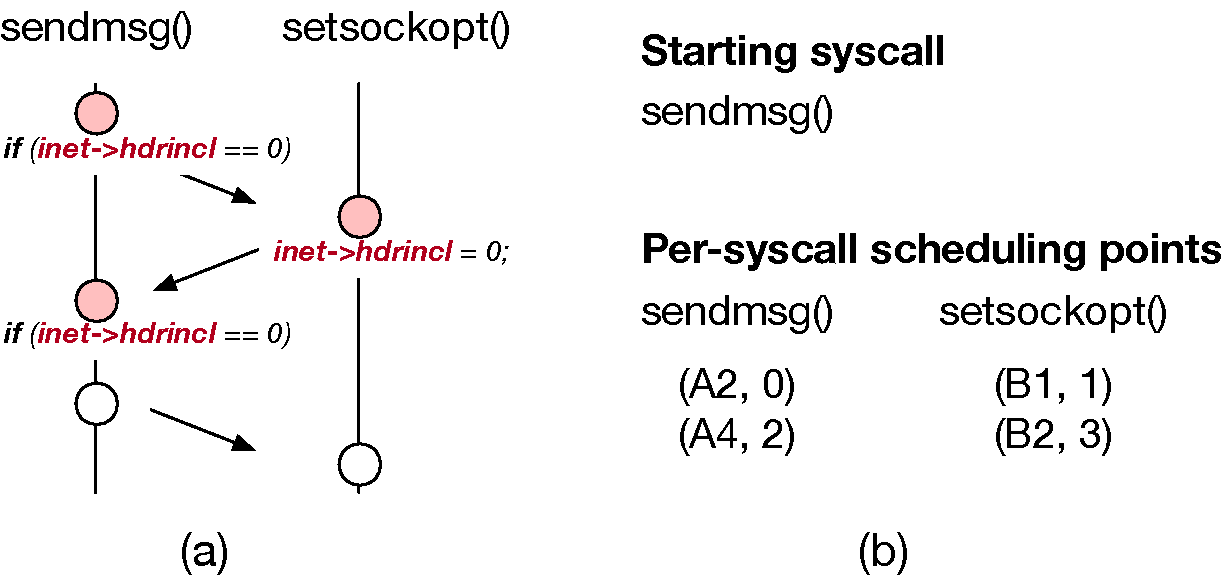
\includegraphics[width=0.75\linewidth]{fig/schedule.pdf}
  \caption{(a) Thread interleaving to run, and (b) schedule describes
    thread interleaving of (a). \dr{redraw (b)}}
  \label{fig:schedule}
\end{figure}

\autoref{fig:schedule} illustrates an example of a schedule. In order
to run a thread interleaving in \autoref{fig:schedule}-(a), the
execution should start with \texttt{sendmsg()}. So the schedule states
that a starting syscall is \texttt{sendmsg()}.
%
Then, in \autoref{fig:schedule}-(a), four preemptions (including the
end of system calls) are required at \texttt{A2}, \texttt{B1},
\texttt{A6}, and \texttt{B2}, and each schedule point denotes on which
these preemptions occur, annotated with the order of preemption.


%During fuzzing, the userspace fuzzer keeps generating different
%schedules, and requests the execution engine through hypercall
%interfaces to control thread scheduling according to a schedule.




\PP{Multi-Thread Generator}
%
% In order to use interleaving graph as interleaving coverage, we need a
% method to store them, and compare them to a new interleaving graph.
% %
% We choose to use a hash value of
%
% the FNV-1~\cite{fnv, fnv-go}, non-cryptographic hash function,
%
%
% A schedule is an outcome of the interleaving mutation.
% A schedule contains an initial thread, and a set of scheduling points
% indicating an instruction on which preemption occurs.
%
The multi-thread generator takes $I_{ST}$, a pair of system calls to run concurrently, and interleaving segment graphs as input. Then, it generates $I_{MT}$ from $I_{ST}$ to


\begin{figure}[t]
  \scriptsize
  \centering
  \begin{Verbatim}[commandchars=\\\{\},codes={\catcode`\$=3\catcode`\^=7\catcode`\_=8\relax}]
\PY{k}{def} \PY{n+nf}{Convert\PYZus{}Pst\PYZus{}to\PYZus{}Pmt}\PY{p}{(}\PY{n}{Pst}\PY{p}{,} \PY{n}{i}\PY{p}{,} \PY{n}{j}\PY{p}{,} \PY{n}{RP\PYZus{}i}\PY{p}{,} \PY{n}{RP\PYZus{}j}\PY{p}{)}\PY{p}{:}
    \PY{c+c1}{\PYZsh{} @Pst: A singled threaded program (annotated)}
    \PY{c+c1}{\PYZsh{} @i, @j: an index of racing syscalls within Pst}
    \PY{c+c1}{\PYZsh{} @RP\PYZus{}i, @RP\PYZus{}j: an address of a corresponding racepair}
    \PY{c+c1}{\PYZsh{} instruction (to syscalls[i] and syscalls[j], respectively)}

    \PY{c+c1}{\PYZsh{} Get pinned threads, thr0 and thr1}
    \PY{n}{thr0} \PY{o}{=} \PY{n}{get\PYZus{}pinned\PYZus{}thread}\PY{p}{(}\PY{n}{vCPU0}\PY{p}{)}
    \PY{n}{thr1} \PY{o}{=} \PY{n}{get\PYZus{}pinned\PYZus{}thread}\PY{p}{(}\PY{n}{vCPU1}\PY{p}{)}

    \PY{c+c1}{\PYZsh{} Assign syscalls to thr0 and thr1}
    \PY{n}{syscalls} \PY{o}{=} \PY{n}{get\PYZus{}syscalls}\PY{p}{(}\PY{n}{Pst}\PY{p}{)}
    \PY{n}{thr0}\PY{o}{.}\PY{n}{add\PYZus{}syscalls}\PY{p}{(}\PY{n}{syscalls}\PY{p}{[}\PY{p}{:}\PY{n}{i}\PY{p}{]}\PY{p}{)}
    \PY{n}{thr1}\PY{o}{.}\PY{n}{add\PYZus{}syscalls}\PY{p}{(}\PY{n}{syscalls}\PY{p}{[}\PY{n}{i}\PY{o}{+}\PY{l+m+mi}{1}\PY{p}{:}\PY{n}{j}\PY{p}{]}\PY{p}{)}

    \PY{c+c1}{\PYZsh{} Determine the execution order}
    \PY{n}{r} \PY{o}{=} \PY{n}{random}\PY{p}{(}\PY{p}{[}\PY{n}{vCPU0}\PY{p}{,} \PY{n}{vCPU1}\PY{p}{]}\PY{p}{)}
    \PY{n}{thr0}\PY{o}{.}\PY{n}{add\PYZus{}hypercall}\PY{p}{(}\PY{n}{hcall\PYZus{}order}\PY{p}{(}\PY{n}{r}\PY{p}{)}\PY{p}{)}

    \PY{c+c1}{\PYZsh{} Trigger and check races}
    \PY{n}{thr0}\PY{o}{.}\PY{n}{add\PYZus{}hypercall}\PY{p}{(}\PY{n}{hcall\PYZus{}set\PYZus{}bp}\PY{p}{(}\PY{n}{vCPU0}\PY{p}{,} \PY{n}{RP\PYZus{}i}\PY{p}{)}\PY{p}{)}
    \PY{n}{thr0}\PY{o}{.}\PY{n}{add\PYZus{}syscalls}\PY{p}{(}\PY{n}{syscalls}\PY{p}{[}\PY{n}{i}\PY{p}{]}\PY{p}{)}
    \PY{n}{thr0}\PY{o}{.}\PY{n}{add\PYZus{}hypercall}\PY{p}{(}\PY{n}{hcall\PYZus{}check}\PY{o}{\PYZhy{}}\PY{n}{race}\PY{p}{(}\PY{p}{)}\PY{p}{)}

    \PY{n}{thr1}\PY{o}{.}\PY{n}{add\PYZus{}hypercall}\PY{p}{(}\PY{n}{hcall\PYZus{}set\PYZus{}bp}\PY{p}{(}\PY{n}{vCPU1}\PY{p}{,} \PY{n}{RP\PYZus{}j}\PY{p}{)}\PY{p}{)}
    \PY{n}{thr1}\PY{o}{.}\PY{n}{add\PYZus{}syscalls}\PY{p}{(}\PY{n}{syscalls}\PY{p}{[}\PY{n}{j}\PY{p}{]}\PY{p}{)}
    \PY{n}{thr1}\PY{o}{.}\PY{n}{add\PYZus{}hypercall}\PY{p}{(}\PY{n}{hcall\PYZus{}check\PYZus{}race}\PY{p}{(}\PY{p}{)}\PY{p}{)}

    \PY{c+c1}{\PYZsh{} Post\PYZhy{}race behaviors}
    \PY{n}{thr0}\PY{o}{.}\PY{n}{add\PYZus{}syscalls}\PY{p}{(}\PY{n}{gen\PYZus{}random\PYZus{}syscalls}\PY{p}{(}\PY{p}{)}\PY{p}{)}
    \PY{n}{thr1}\PY{o}{.}\PY{n}{add\PYZus{}syscalls}\PY{p}{(}\PY{n}{gen\PYZus{}random\PYZus{}syscalls}\PY{p}{(}\PY{p}{)}\PY{p}{)}

    \PY{n}{Pmt} \PY{o}{=} \PY{n}{Construct\PYZus{}Pmt}\PY{p}{(}\PY{n}{thr0}\PY{p}{,} \PY{n}{thr1}\PY{p}{)}
    \PY{k}{return} \PY{n}{Pmt}
\end{Verbatim}

  \caption{\sys's multi-thread generator algorithm}
  \label{f:mt-conversion}
\end{figure}




\PP{Multi-Thread Executor}
%
The purpose of the multi-thread executor is to run $I_{MT}$ while
enforcing a schedule generated by the multi-thread generator.
%
To this end, the multi-thread executor gets support from the execution
engine~(\autoref{ss:engine}), which enforces thread scheduling
according to a given schedule.


While controling thread scheduling

In addition, the multi-thread executor detects a concurrency bug with
various dynamic tools such as lockdep~\cite{lockdep}, and
KAsan~\cite{kasan}.



During the execution of $I_{MT}$,

For example, the Linux
kernel employs various dynamic techniques to detect harmful
races. Examples are lockdep [29], KASAN [2], or assertions
manually inserted by kernel developers. We enabled all of
these techniques while building the kernel binary such that
RAZZER can leverage this enhanced race detection capability.
If a violation is detected, RAZZER generates a detailed report
about the harmful race.

After executing $I_{MT}$, the multi-thread executor collect memory accesses that racing system calls executed.
%
With these memory accesses, it tracks interleaving segment coverage.








\subsection{Target Kernel Instrumentation}
\label{ss:instrumentation}

\sys requires to trace basic blocks (for code coverage) and memory
accesses (for interleaving coverage) executed by each system call.
%
To this end, \sys incorporates a compiler pass that inserts callback
function calls 1) at the beginning of each basic block, and 2) before
each instruction that accesses globally-visible memory objects.
%
These callback functions records executed basic blocks and memory
accesses into memory regions shared between the user space and the
kernel space.



\begin{figure}
  \centering
  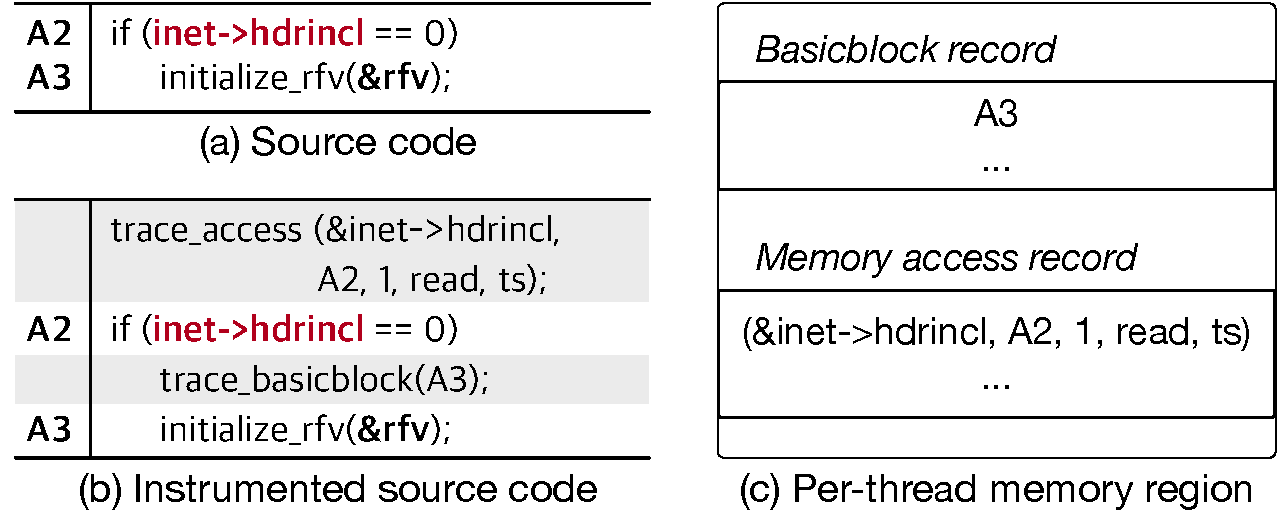
\includegraphics[width=0.9\linewidth]{fig/instrumentation.pdf}
  \caption{(a) Part of \texttt{raw_sendmsg()} in
    \autoref{fig:cve-2017-17712}, (b) instrumented source code of (a)
    (gray on the background), and (c) memory accesses and basic blocks
    recorded during runtime.}
  \label{fig:instrumentation}
\end{figure}

\autoref{fig:instrumentation} shows how the \sys's compiler pass
inserts callbacks, and how each callback records memory accesses and
basic blocks.
%
When compiling a source code in (a), the compiler pass two inserts
function calls; \texttt{trace_basicblock()} before \texttt{A3} which
is the first instruction of the basic block, and
\texttt{trace_access()} before \texttt{A2} which is an instruction
that accesses \texttt{inet->hdrincl}.


During runtime, \texttt{trace_basicblock()} takes the starting address
of basic block as input (\ie, \texttt{A3}), and records the starting
address into \texttt{Basicblock record}.
%
On the other hand, \texttt{trace_access()} takes four parameters, the
address of the accessed memory object (\ie, \texttt{\&inet->hdrincl}),
the instruction address accessing the memory object (\ie,
\texttt{A2}), the size of the memory access (\ie, \texttt{1}), and
the type of the memory access (\ie, \texttt{read}), and records them
into \texttt{Memory access record}.






It is worth noting that \texttt{Basicblock record} and \texttt{Memory
  access record} are per-thread memory regions, shared between the
user space and the kernel space. Thus, after a userspace thread
executes a system call, the thread can identify basic blocks and
memory accesses that it executed.







% Unlike data race detectors such as KCSAN~\cite{kcsan}, the \sys's
% scheduling mechanism needs to recognize both plane memory accesses and
% annotated memory accesses such as atomic operations.
% %
% We deal with these two types of accesses differently since annotated
% accesses usually are implemented in assembly code, which is hard for a
% LLVM pass to understand.
% %
% In order to instrument plane accesses, we implement a LLVM pass that
% insert callback function calls after memory accesses on LLVM IR.
% %
% Our pass runs after most of binary transfomration is done, so it
% \XXX{...}.
% %
% For annotated instructions, we rely on the functionality of
% KASAN~\cite{kasan} to instrument atomic operations.
% %
% KASAN provides wrapper functions of annotation APIs to call callback
% functions before annotated memory operations, and we instruct the
% wrapper functions to call our callbacks as well.
% %
% Our callbcak functions write memory access operations along with
% various information into a region mmap-ed shared region shared by a
% userspace program (\ie, fuzzer) and a kernel. The information about
% memory operations includes the instruction address, the start address
% of a memory location, and the size of memory access.
% %
% Accordingly, a fuzzer is able to identify what memory access
% operations took place during the execution.

% \sys also requires an additional module called a trampoline that is
% used to suspend and resume a running thread. Details about the
% trampoline are described in \autoref{ss:engine}.


\subsection{Execution Engine}
\label{ss:engine}

\sys introduces an execution engine in order to grant an ability to
the userspace fuzzer that it can control thread scheduling.
%
The execution engine is implemented in the hypervisor layer to be
non-intrusive to the kernel execution, and the userspace fuzzer can
request the execution engine to control thread scheduling through
hypercall interfaces.





\PP{Workflow of enforcing a schedule}
%
In order for the userspace fuzzer to ask the execution engine to
enforce a schedule, the userspace fuzzer sends a schedule to run
thorugh hypercall interfaces.
%
After that, the threads notify the execution engine that they are
ready to execute system calls, and start executing system calls,
%
During the execution, the execution engine keeps only one thread to
run, and deliberately suspends and resumes the execution of system
calls according to the given schedule.

%
\begin{figure}[t]
  \centering
  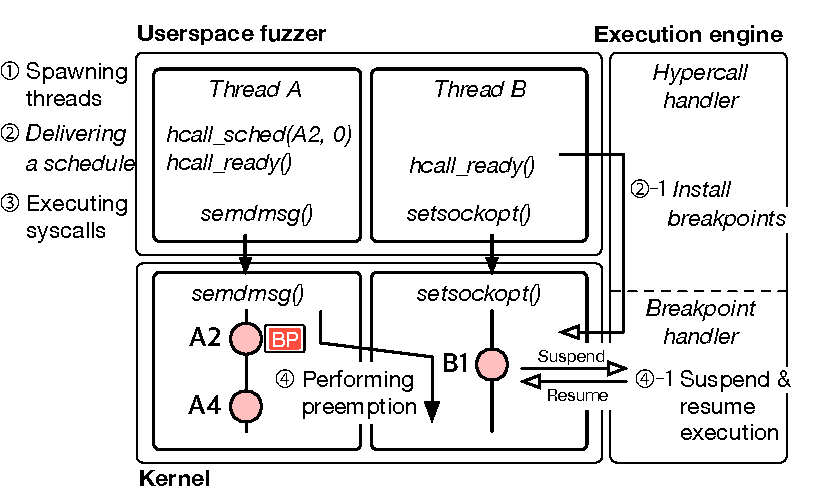
\includegraphics[width=0.9\linewidth]{fig/workflow-hypervisor.pdf}
  \caption{The workflow of the execution engine. \red{IMPORTANT: this
      is copied from AITIA. Need to redraw}}
  \label{fig:workflow-hypervisor}
\end{figure}
%
\autoref{fig:workflow-hypervisor} shows a workflow of the execution
engine.
%
At the beginning, the userspace fuzzer spawns threads, where each
thread is assigned a system call annotated with scheduling points.
%
Then, each thread invokes hypercalls (\ie,
\texttt{hcall_scheduling_point()}) to deliver scheduling points to the
execution engine, followed by a hypercall \texttt{hcall_ready()} that
sleeps until all threads are ready.
%
After all threads invoke \texttt{hcall_ready()}, the execution engine
wakes them up, and the threads start executing system calls.


\dr{}



\PP{Performing preemption}
%
In order to perform preemption, \sys leverages the hardware breakpoint
feature~\cite{hwbp} shipped in modern Intel CPU chipsets.
%
When the execution engine receives scheduling points, the execution
engine installs breakpoints on instructions on which scheduling points
refer, and recognizes that a thread of the userspace fuzzer reaches a
scheduling point when a breakpoint is hit.


When a thread hits a breakpoint, the execution engine saves register
values of the thread, and then changes the program counter of the
thread to an infinite loop called a trampoline.
%
In the trampoline, the thread keeps calling \texttt{cond_resched()} to
yield a CPU without proceeding with the system call execution.
%
To resume the suspended thread, the execution engine restores
registers with the values of registers including a program counter
saved when the thread was suspended, and then the thread can continue
its execution.


\PP{Restriction of hardware breakpoint}
%
While a hardware breakpoint feature is well-fitting for our pupose, it
has a restriction on the number of breakpoints that can be installed
at the same time.
%
In Intel CPU chipsets, at most four hardware breakpoints can be
installed simultaneously, and the number of scheduling points can be
larger than four.
%
\sys overcomes this restriction by leveraging the fact that
scheduling points are ordered. In other words, the execution engine
installs breakpoints on a first few (\eg, four) scheduling points,
and when a installed breakpoint is hit, the execution engine moves a
breakpoint onto the next scheduling point.
%
Also we expect that this restriction can be further mitigated by using
architectures with more hardware breakpoints (\eg, ARM v7 equipped six
hardware breakpoints), or using a software breakpoint feature that
does not have a restriction on the number of breakpoints.



%\dr{not important. i'm thinking remove this}
%
%In performing preemption, we choose to suspend and resume a guest
%thread instead of a whole virtual CPU on which the guest thread runs.
%
%While suspending and resuming a whole virtual CPU is adopted by
%previous approaches~\cite{ski, snowboard, razzer} it is not suitable
%for our purpose because \textit{if suspending a virtual CPU, it may
%  suspend another virtual CPU}. Details are explained in the appendix
%section~(\autoref{s:appendix:preemption}).




\PP{Handling missing scheduling points}
%
It is worth noting that instructions on which scheduling points
install may not be executed if the control flow changes due to kernel internal states.
%
\dr{}In such case, we keep the order of scheduling points.
%
For example, when executing a schedule of \autoref{fig:schedule}, it is possible that thread~A may not execute \texttt{A2}, and hit a breakpoint on \texttt{A6}.
%
Then, we ignore all scheduling points before \texttt{A6} (\ie, \texttt{A2} and \texttt{B1}), and keep
enforcing a schedule after \texttt{A6} (\ie, \texttt{B2}).



\PP{Virtual Machine Instrospection}
%
While controlling thread scheduling of system calls, the execution
engine introspects the target kernel for two reasons.
%
First, because a hardware breakpoint does not distinguish which thread
hits the breakpoint, the execution engine needs to determine whether
the breakpoint is hit by a thread of the userspace fuzzer, or by an
irrelevant thread.
%
If a breakpoint is hit by a thread of the userspace fuzzer, the
execution engine suspends the thread and resumes the
previously-suspended thread as specified in a schedule.
%
Otherwise, the execution engine ignores the breakpoint hit, and keeps
running the kernel.


Second, when a running thread tries to acquire a lock, the execution
engine inspects whether the lock is held by a suspended thread to
prevent unexpected block (\ie, both threads cannot make a progress).
%
If it is the case, the execution engine performs preemption so that
the lock-holder thread (\ie, the suspended thread) resumes the
execution, and the lock-waiting thread gets suspended.


While the virtual machine introspection is crucial to properly control
thread scheduling, we leave details of how we implement the virtual
machine introspection in the appendix
section~(\autoref{s:appendix:vmi}).




\subsection{Implementation}
\label{ss:impl}

We implement \sys in various software layers as follows:
%
The target kernel instrumentation~(\autoref{ss:instrumentation}) is
implemented in two parts, a compiler pass and callback functions. The
compiler pass is implemented on the LLVM compiler suite
12.0.1~\cite{llvm} by modifying two existing LLVM passes, the
\texttt{SanitizerCoverage} pass~\cite{kcovpass} (for tracing basic
blocks) and the \texttt{ThreadSanitizer} pass~\cite{tsanpass} (for
tracing memory accesses).
%
And, the callback functions are implemented in the Linux kernel source
tree.
%
Thus, when compiling the kernel, our callbacks are also compiled into
the kernel binary.


The execution engine~(\autoref{ss:engine}) is implemented on QEMU
6.0.0, and leverages KVM (Kernel-based Virtual Machine) to take
advantage of hardware acceleration.
%
To allow hypercalls from the guest user space, we also modify the KVM
module of the host kernel.
%
In addition, the trampoline is enclosed into the target kernel source
tree as a loadable module.


Lastly, the \sys's userspace fuzzer~(\autoref{ss:fuzzer}) is
implemented based on \texttt{Syzkaller}~\cite{syzkaller}, a kernel
fuzzer developed by Google.



\PP{Lines of Code}
%
We use scc~\cite{scc} and sloccount~\cite{sloccount} to measure LoC of
GO and C, C++ respectively.
%
To summarize, the target kernel
instrumentation~(\autoref{ss:instrumentation}) is implemented with 323
LoC in C++ (for the compiler pass) and 265 LoC in C (for callback
functions).
%
The execution engine~(\autoref{ss:engine}) is implemented with 1662
LoC in C. And the userspace fuzzer~(\autoref{ss:fuzzer}) is
implemented with 3334 LoC in GoLang and 341 LoC in C++.

% the compiler pass is implmented in 323 lines of C++
% the callback functions are implmeneted in 265 lines of C
% the execution engine is implemented in 1662 lines of C
% the trampoline is 66 in C
% c2fuzz:
% go 3334
% C++ 341







%%% Local Variables:
%%% mode: latex
%%% TeX-master: "p"
%%% End:
